% Pages 174–200: Morin 2.6, Introduction to Lagrangian Mechanics,
% Calculus of Variations, Particle Interactions, Symmetry & Noether's Theorem,
% Non-Inertial Reference Frames, Double Pendulum

\chapter{Introduction to Lagrangian Mechanics}

% -----------------------------------------------------------------------
\section{Morin Problem 2.6 (Rope over a Pulley)}

A small element of rope subtending an angle $d\theta$ at angular position $\theta$
is acted on by tension forces $T(\theta + d\theta/2)$ and $T(\theta - d\theta/2)$
and a normal force $dN$ directed toward the center of the pulley.

\begin{figure}[H]
    \centering
    \caption{Rope element on a circular pulley. The element subtends angle $d\theta$;
    tension acts at $\pm d\theta/2$ from the element centre and a normal force $dN$
    acts radially inward.}
\end{figure}

Horizontal (tangential) equilibrium gives
\[
    T\!\left(\theta + \tfrac{d\theta}{2}\right)\cos\!\left(\tfrac{d\theta}{2}\right)
    =
    T\!\left(\theta - \tfrac{d\theta}{2}\right)\cos\!\left(\tfrac{d\theta}{2}\right).
\]

The vertical (normal) component of the net tension is
\[
    dN_y = 2T\sin\!\left(\tfrac{d\theta}{2}\right)\cos\theta = T\cos\theta\,d\theta.
\]

Boundary conditions: $dN_y = 0$ when $\theta = \tfrac{\pi}{2}, -\tfrac{\pi}{2}$.

Integrating,
\[
    N_y = T(\sin\theta_f - \sin\theta_i) = 2T.
\]

But $N_y = Mg$, so
\[
    \boxed{T = \frac{Mg}{2}.}
\]

\textit{Easier way:} $Mg = 2T$.  The normal force per unit length is the same
everywhere:
\[
    dN = N\,d\theta = 2T\sin\!\left(\tfrac{d\theta}{2}\right) = T\,d\theta.
\]

Since the $N\,d\theta/dN$ segment has arc length $R\,d\theta$,
\[
    \boxed{\frac{N}{R} = \frac{T}{R} = \frac{Mg}{2R}.}
\]

\subsection*{Part (b)}

Use the result that $T(\theta) \leq T(0)\,e^{\mu\theta}$.

% -----------------------------------------------------------------------
\section{Motivation}

\textit{(Lecture: Introduction to Lagrangian Mechanics, Monday January 6, 2025)}

\subsection{Newtonian Picture}

Given initial conditions $\vec{x}(t=0)$ and $\dot{\vec{x}}(t=0)$, Newton's laws
tell you how to update the system:
\[
    \vec{a} \;\to\; \vec{v} \;\to\; \vec{x}, \qquad m\ddot{\vec{x}} = \sum_i \vec{F}_i.
\]

\begin{itemize}
    \item Q: Where do Newton's laws come from? Why are certain quantities conserved?
\end{itemize}

\subsection{Motivation: Refraction and Fermat's Principle}

How does light know which path to take through a block?

\begin{itemize}
    \item \textbf{Fermat's Principle:} The path that takes the least time is the one
        that light chooses to take.
\end{itemize}

\begin{figure}[H]
\begin{center}
\begin{tikzpicture}[scale=1.0, >=Stealth]
  % Interface
  \draw[thick,dashed] (-1.5,0) -- (3.0,0);
  % Media labels
  \node[above left] at (-1.0,0.8) {$n_1$ (medium 1)};
  \node[below left] at (-1.0,-0.5) {$n_2$ (medium 2)};
  % Fill media
  \fill[blue!8] (-1.5,0) rectangle (3.0,2.0);
  \fill[orange!8] (-1.5,-1.5) rectangle (3.0,0);
  % Incident ray
  \draw[->,thick,blue] (-1.0,1.8) -- (1.0,0);
  % Refracted ray
  \draw[->,thick,red] (1.0,0) -- (2.5,-1.3);
  % Normal line
  \draw[dashed,gray] (1.0,1.5) -- (1.0,-1.2);
  % Angle theta1
  \draw (1.0,0.7) arc[start angle=90,end angle=118,radius=0.7];
  \node[left,scale=0.85] at (0.7,0.85) {$\theta_1$};
  % Angle theta2
  \draw (1.0,-0.6) arc[start angle=270,end angle=302,radius=0.6];
  \node[right,scale=0.85] at (1.2,-0.7) {$\theta_2$};
  % Snell label
  \node[right] at (2.6,-0.4) {$n_1\sin\theta_1 = n_2\sin\theta_2$};
\end{tikzpicture}
\end{center}
\caption{Snell's law from Fermat's principle: light refracts at the interface between media with speeds $v_1 = c/n_1$ and $v_2 = c/n_2$. The path of least time gives $n_1\sin\theta_1 = n_2\sin\theta_2$.}
\label{fig:fermat_snell}
\end{figure}

Is there some quantity that is optimised?

\subsection{Hamilton's Picture}

Assume we know the position at an initial and final time.  Is there a principle
that allows you to discern the path?

\begin{figure}[H]
\begin{center}
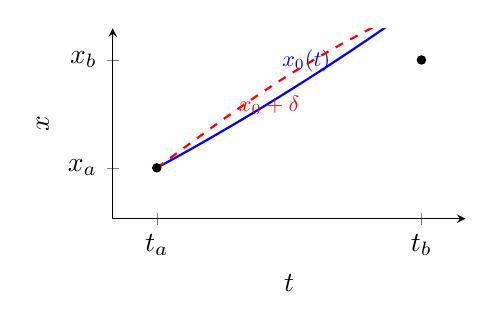
\begin{tikzpicture}
\begin{axis}[
  width=0.5\textwidth, height=4cm,
  xlabel={$t$}, ylabel={$x$},
  xmin=0, xmax=4, ymin=0, ymax=3,
  xtick={0.5,3.5}, xticklabels={$t_a$,$t_b$},
  ytick={0.8,2.5}, yticklabels={$x_a$,$x_b$},
  axis lines=left,
]
  % True path (parabola)
  \addplot[thick,blue,domain=0.5:3.5,samples=50]
    {0.8 + 0.75*(x-0.5) + 0.04*(x-0.5)^2} node[pos=0.55,above,scale=0.8]{$x_0(t)$};
  % Varied path (different curve)
  \addplot[thick,dashed,red,domain=0.5:3.5,samples=50]
    {0.8 + 0.75*(x-0.5) + 0.04*(x-0.5)^2 + 0.25*sin(deg(pi*(x-0.5)/3))}
    node[pos=0.45,below,scale=0.8]{$x_0+\delta$};
  % Endpoint marks
  \addplot[only marks,mark=*,mark size=1.5pt] coordinates {(0.5,0.8)(3.5,2.5)};
\end{axis}
\end{tikzpicture}
\end{center}
\caption{The true (classical) path $x_0(t)$ (blue solid) and a varied path $x_0(t)+\delta(t)$ (red dashed) between fixed endpoints $(t_a,x_a)$ and $(t_b,x_b)$. Hamilton's principle states $\delta S = 0$ for the true path.}
\label{fig:action_paths}
\end{figure}

% -----------------------------------------------------------------------
\section{First Principles}

\begin{enumerate}
    \item Inertial reference frames exist, and in them the CoM of an isolated system
        experiences no acceleration \textit{(1st Law)}.
    \item Space-time is homogeneous and isotropic — the fundamental laws of physics
        don't depend on time or location.
        \begin{itemize}
            \item Box experiment: chiral particles?
            \item Hyperfine splitting
        \end{itemize}
\end{enumerate}

\textit{Implicit assumptions:}
\begin{enumerate}
    \item[(a)] Time is absolute; fundamental interactions are instantaneous.
    \item[(b)] Nature is deterministic.
    \item[(c)] There are no (interaction-dependent) fundamental constants of nature
        (e.g.\ $c$, $\hbar$, etc.).
\end{enumerate}

% -----------------------------------------------------------------------
\section{The 1-D Point Particle and the Action}

\begin{figure}[H]
\begin{center}
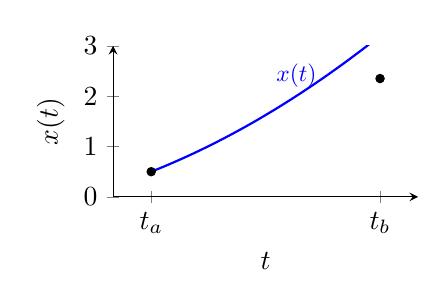
\begin{tikzpicture}
\begin{axis}[
  width=0.45\textwidth, height=3.5cm,
  xlabel={$t$}, ylabel={$x(t)$},
  xmin=0, xmax=4, ymin=0, ymax=3,
  xtick={0.5,3.5}, xticklabels={$t_a$,$t_b$},
  ytick={}, axis lines=left,
]
  \addplot[thick,blue,domain=0.5:3.5,samples=60]
    {0.5+0.6*(x-0.5)+0.1*(x-0.5)^2} node[pos=0.6,above,scale=0.85]{$x(t)$};
  \addplot[only marks,mark=*,mark size=1.5pt] coordinates {(0.5,0.5)(3.5,2.35)};
\end{axis}
\end{tikzpicture}
\end{center}
\caption{The path $x(t)$ of a 1-D particle between fixed endpoints at times $t_a$ and $t_b$. The Lagrangian $L(x,\dot{x},t)$ characterises how each path is weighted by the action $S = \int_{t_a}^{t_b} L\,dt$.}
\label{fig:1d_path}
\end{figure}

\begin{itemize}
    \item Assume there is some function $L(x, \dot{x}, t)$ that in some way
        characterises the path.
    \item We can't find $L$ with a finite number of points (infinite number of paths
        go through any finite set of points).
\end{itemize}

Therefore we must look at the \textbf{action}:
\[
    S = \int_{t_a}^{t_b} L(x, \dot{x}, t)\,dt + C
    + \underbrace{\int_{t_a}^{t_b} \dv{t}\!\left[f(x,t)\right]dt}_{\text{total time derivative — set to 0}}.
\]

$S$ is a \textbf{functional}: a function of a function $x(t)$.

\begin{itemize}
    \item \textbf{Assertion 1:} Any additive constant $C$ can be set to 0 (analogous
        to the constant in a potential).
    \item \textbf{Assertion 2:} The red (total-derivative) term is also constant if it
        is the integral of a derivative of some function of time (e.g.\ $2t^2$).
\end{itemize}

\subsection{Examining the Postulates}

\begin{itemize}
    \item \textbf{Postulate 1:} $\dot{x} \to \dot{x} + V$ (Galilean transformation).
        In both frames the physics is the same $\Rightarrow \delta S = 0$ (up to a
        constant) $\Rightarrow$ path can't change meaningfully.
    \item \textbf{Postulate 2:}
        \begin{itemize}
            \item $t + \delta t \Rightarrow \delta S = 0$ (equations of motion must be
                time-translation invariant).
            \item $x + \delta x \Rightarrow \delta S = 0$ (space-translation invariance).
            \item $x \to -x$ $(\dot{x} \to -\dot{x}) \Rightarrow \delta S = 0$
                (rotation invariance).
        \end{itemize}
\end{itemize}

\subsection{Determining the Free Lagrangian}

Define $L_\mathrm{Free}^{1\text{-D}} \equiv K(x, \dot{x}, t)$.

\begin{itemize}
    \item $K$ cannot have pure terms that are functions of $t$ alone (from Assertion 2).
    \item $x \to -x \Rightarrow \delta S = 0 \Rightarrow K(-x, -\dot{x}, t) = K(x, \dot{x}, t)$.
    \item Try a polynomial: $K = C_0 + C_2 x^2 + C_4 x^4 + C_{-2}x^{-2} + \cdots$
    \item $x \to x + \delta x \Rightarrow \delta S = 0 \Rightarrow x^2 \to (x+\delta x)^2
        = x^2 + \underbrace{\delta x^2}_{\text{const. so far}} + \underbrace{2\delta x\, x}_{\text{not const.}}$
        \textbf{Problem!}
    \item \textbf{No pure functions of $x$ work!}
\end{itemize}

Try $K = C_2 \dot{x}^2 + C_4 \dot{x}^4 + \cdots$:
\begin{align*}
    (\dot{x} + V)^2 &= \dot{x}^2 + V^2 + 2\dot{x}V = \dot{x}^2 + \dv{t}[2Vx] \checkmark \\
    (\dot{x} + V)^4 &= \dot{x}^4 + V^4 + 4\dot{x}^3 V + 6V^2\dot{x}^2 + 4V\dot{x}^3 \;\times
        \quad \text{(cannot be written as a total derivative)}
\end{align*}

\begin{itemize}
    \item The only function that works is $K(\dot{x}) = C\dot{x}^2$.
    \item Because the only intrinsic property of a point particle is its mass,
        \[
            K(\dot{x}) = \alpha(m)\,m\dot{x}^2.
        \]
    \item Assume $K(\dot{x})$ has units of $[E]$, so $\alpha(m)$ is dimensionless.
\end{itemize}

\begin{figure}[H]
    \centering
    \caption{The action $S$ as a functional of the path. The minimum (orange dot)
    corresponds to the physical path. When $\dot{x} \to \dot{x}+V$, $S$ translates
    up and down, so neither absolute values of $S$ nor $\Delta S$ matter (different
    units).}
\end{figure}

$S$ has units of $[\text{J}][\text{s}]$.

\begin{itemize}
    \item Different inertial frames should agree on extremum points.
    \item Paths that are similar are close; paths that are different are far apart.
\end{itemize}

% -----------------------------------------------------------------------
\section{Extremising the Action: Euler–Lagrange Equation}

We want
\[
    S[x_0(t) + \delta(t)] - S[x_0(t)] = 0.
\]

Notice $\delta(t_a) = \delta(t_b) = 0$.

Take a Taylor expansion of $\delta S$:
\[
    \delta S = 0 = \int_{t_a}^{t_b}
    \left[\frac{\partial L}{\partial x}(x - x_0)
    + \frac{\partial L}{\partial \dot{x}}(\dot{x} - \dot{x}_0)\right]dt.
\]

Note that
\[
    \dv{t}\!\left[\frac{\partial L}{\partial \dot{x}}\,\delta\right]
    = \frac{\partial L}{\partial \dot{x}}\,\dot{\delta}
    + \left[\dv{t}\frac{\partial L}{\partial \dot{x}}\right]\delta.
\]

Replacing the $\frac{\partial L}{\partial \dot{x}}\dot{\delta}$ term:
\[
    \Rightarrow \int_{t_a}^{t_b} dt\,\delta\!\left[
        \frac{\partial L}{\partial x} - \dv{t}\frac{\partial L}{\partial \dot{x}}
    \right]
    + \left[\frac{\partial L}{\partial \dot{x}}\,\delta\right]_{t_a}^{t_b} = 0.
\]

The boundary term vanishes because $\delta(t_a) = \delta(t_b) = 0$.

\begin{formula}[Euler--Lagrange Equation]
    \[
        \boxed{\frac{\partial L}{\partial x} - \dv{t}\frac{\partial L}{\partial \dot{x}} = 0}
    \]
\end{formula}

Substituting $L = \alpha(m)\,m\dot{x}^2$:
\[
    \frac{\partial L}{\partial x} - \dv{t}\frac{\partial L}{\partial \dot{x}}
    = 0 - \dv{t}\!\left[2\alpha(m)\,m\dot{x}\right] = 0
    \;\Rightarrow\; \dot{x} = \text{const.}
\]

This is Newton's First Law for a free particle.

% -----------------------------------------------------------------------
\section{Two-Particle System}

\begin{figure}[H]
    \centering
    \caption{Two particles on a line, with positions $x_1$, $x_2$, velocities
    $\dot{x}_1$, $\dot{x}_2$, and masses $m_1$, $m_2$.}
\end{figure}

Now
\[
    S = \int_{t_a}^{t_b} L(x_1, \dot{x}_1, x_2, \dot{x}_2, t)\,dt.
\]

Once again assume $\delta_i(t_a) = \delta_i(t_b) = 0$ for $i = 1, 2$.  Then
\[
    \delta S = 0 \Rightarrow
    \int_{t_a}^{t_b} dt \left[
        \frac{\partial L}{\partial x_1}(x_1 - x_1^0)
        + \frac{\partial L}{\partial \dot{x}_1}(\dot{x}_1 - \dot{x}_1^0)
        + \frac{\partial L}{\partial x_2}(x_2 - x_2^0)
        + \frac{\partial L}{\partial \dot{x}_2}(\dot{x}_2 - \dot{x}_2^0)
    \right] = 0.
\]

You can set $\delta_1 = 0$ to examine $\delta_2$, and vice versa, because they must
work for all $\delta_1, \delta_2$.  Therefore
\[
    L_\mathrm{Free}^{1\text{-D}}
    = K(\dot{x}_1) + K(\dot{x}_2)
    = \alpha(m_1)\,m_1\dot{x}_1^2 + \alpha(m_2)\,m_2\dot{x}_2^2.
\]

% -----------------------------------------------------------------------
\chapter{Calculus of Variations}

\textit{(Recitation 1: Review of Calculus of Variations, Monday January 6, 2025)}

\section{Total vs.\ Partial Derivatives}

Suppose $f(t, x(t), y(t)) : \mathbb{R} \to \mathbb{R}$.

\subsection{Partial Derivative $\partial f / \partial t$}

Assume all variables fixed, except $t$.

\begin{example}[Partial Derivative]
    \[
        f(t, x, y) = t^3 + 2x + 3ty
        \;\Rightarrow\;
        \frac{\partial f}{\partial t} = 3t^2 + 0 + 3y.
    \]
\end{example}

In general, for $f(\vec{x}(t))$ where $\vec{x}(t) = (x_1(t), x_2(t), \ldots, x_n(t))$:

\begin{formula}[Total Derivative]
    \[
        \dv{f}{t} = \sum_{i=1}^{N} \frac{\partial f}{\partial x_i}\dv{x_i}{t}.
    \]
\end{formula}

For $f(t, x(t), y(t))$ where $x, y$ are also functions of $t$:
\[
    \dv{f}{t}
    = \frac{\partial f}{\partial t}\cdot\frac{\partial t}{\partial t}
    + \frac{\partial f}{\partial x}\frac{\partial x}{\partial t}
    + \frac{\partial f}{\partial y}\frac{\partial y}{\partial t}.
\]

\begin{example}[Total Derivative]
    \[
        \dv{f}{t} = 3t^2 + 3y + 2\dot{x} + 3t\dot{y}.
    \]
\end{example}

\subsection{Local and Convective Derivative}

For $f(t) = f(t, x(t), y(t), z(t))$:
\[
    \dv{f}{t}
    = \frac{\partial f}{\partial t}
    + \frac{\partial f}{\partial x}\frac{\partial x}{\partial t}
    + \frac{\partial f}{\partial y}\frac{\partial y}{\partial t}
    + \frac{\partial f}{\partial z}\frac{\partial z}{\partial t}.
\]

The velocity vector is $\vec{v} = (\dot{x}, \dot{y}, \dot{z})$ and the gradient is
$\nabla f = \frac{\partial f}{\partial x}\hat{x} + \frac{\partial f}{\partial y}\hat{y}
+ \frac{\partial f}{\partial z}\hat{z}$.  Thus
\[
    \dv{f}{t}
    = \underbrace{\frac{\partial f}{\partial t}}_{\text{local derivative}}
    + \underbrace{\vec{v}\cdot\nabla f}_{\text{convective derivative}}.
\]

% -----------------------------------------------------------------------
\section{Calculus of Variations}

The action $S[f(t,\vec{q})]$ is a \textbf{functional}: input a function, output a
scalar, where $S : (f[\mathbb{R}, \mathbb{R}]) \to \mathbb{R}$.

\begin{example}[General Functional]
    \[
        J[y_i] = \int_{x_1}^{x_2} dx\; F\!\left(y_1(x), \ldots, y_N(x),\,
        y_1'(x), \ldots, y_N'(x),\, x\right).
    \]
    $y_i(x)$ can be maximised, minimised, or set to 0.
\end{example}

\textbf{Calculus of Variations (CoV):} Want a set of functions that extremise the
functional, i.e.\ $\delta J = 0$.

\begin{itemize}
    \item Use small variations to find maxima/minima of our functional $J$.
    \item Consider $y_i^* = y_i(x) + \delta y_i(x)$ where
        $|\delta y_i(x)| \ll |y_i(x)|$, $|\delta y_i'| \ll y_i'(x)$.
    \item Constraint: $\delta y(x_1) = \delta y(x_2) = 0$,
        $\delta y'(x_1) = \delta y'(x_2) = 0$.
\end{itemize}

\begin{figure}[H]
    \centering
    \caption{The extremal path $y_i(x)$ and a neighbouring varied path $y_i^*$ between
    fixed endpoints $x_1$ and $x_2$.}
\end{figure}

\subsection{Computing the Variation}

\[
    \delta J = J[y + \delta y] - J[y]
    = \int_{x_1}^{x_2} F\!\left[y+\delta y,\;\frac{dy}{dx}+\delta\frac{du}{dx},\;x\right]dx
    - \int_{x_1}^{x_2} F\!\left[y,\;\frac{dy}{dx},\;x\right]dx.
\]

Write the first integrand as a Taylor series.

\subsubsection{Taylor Series}

\[
    F(x, y) \approx F(x_0, y_0)
    + (x - x_0)\left.\frac{\partial F}{\partial x}\right|_{\substack{x=x_0\\y=y_0}}
    + (y - y_0)\left.\frac{\partial F}{\partial y}\right|_{\substack{x=x_0\\y=y_0}}
    + O(\delta^2).
\]

Let $y_0 = y$, $y_0' = y'$, so
\[
    F(y+\delta y,\; y'+\delta y',\; x)
    \approx F(y, y', x) + (\delta y)\frac{\partial F}{\partial y}
    + \delta y'\frac{\partial F}{\partial y'} + O(\delta^2).
\]

Therefore
\begin{align*}
    \delta J
    &= \int_{x_1}^{x_2} dx\left[F(y,y',x) + \frac{\partial F}{\partial y}\delta y
       + \frac{\partial F}{\partial y'}\delta y'\right]
     - \int_{x_1}^{x_2} dx\left[F(y,y',x)\right] \\
    &= \int_{x_1}^{x_2} dx\left[\frac{\partial F}{\partial y}\delta y
       + \frac{\partial F}{\partial y'}\delta y'\right].
\end{align*}

Integrate the second term by parts ($\int u\,dv = uv - \int v\,du$):
\[
    \int_{x_1}^{x_2} dx\left(\frac{\partial F}{\partial y'}\right)\delta y'
    = \left.\frac{\partial F}{\partial y'}\delta y\right|_{x_1}^{x_2}
    - \int_{x_1}^{x_2} \delta y \cdot \dv{x}\!\left(\frac{\partial F}{\partial y'}\right)dx.
\]

(Here $u = \partial F/\partial y'$ and $dv = \delta y'\,dx$.)

\[
    \Rightarrow\;
    \delta J = \int_{x_1}^{x_2} dx\left[
        \frac{\partial F}{\partial y} - \dv{x}\!\left(\frac{\partial F}{\partial y'}\right)
    \right]\delta y \;\neq 0.
\]

\[
    \Rightarrow\; \delta J = 0
    \;\Rightarrow\;
    \frac{\partial L}{\partial q} - \dv{t}\!\left(\dv{L}{\dot{q}}\right) = 0
\]

with the substitution $F \to L$, $J \to S$, $x \to t$.

% -----------------------------------------------------------------------
\chapter{Particle Interactions and Example Usage}

\textit{(Lecture: Particle Interactions and Example Usage, Tuesday January 7, 2025)}

\section{From Last Time}

\[
    L_\mathrm{Free}^{1\text{-D}}
    = \alpha(m_1)\,m_1\dot{x}_1^2 + \alpha(m_2)\,m_2\dot{x}_2^2,
    \quad \text{has dimensions of } E.
\]

% -----------------------------------------------------------------------
\section{Conservative Interactions}

\begin{itemize}
    \item Work done by a force is path-independent.
    \item $\vec{F} = -\nabla\phi$ — force is the negative gradient of a potential.
\end{itemize}

\[
    L = L_\mathrm{Free}^{1\text{-D}} + \mathcal{I}(x_1, x_2).
\]

Applying the postulates again:
\begin{itemize}
    \item $x_i \to x_i + \delta x_i \Rightarrow \delta S = 0$:
        this means $\mathcal{I}$ must depend on $x_1 - x_2$ (invariant to translation).
    \item $x_i \to -x_i \Rightarrow \delta S = 0$:
        this means $\mathcal{I}$ depends on $|x_1 - x_2|$ (depends on distance).
\end{itemize}

Let $\Delta x \equiv |x_1 - x_2|$.
\[
    L = \alpha(m_1)\,m_1\dot{x}_1^2 + \alpha(m_2)\,m_2\dot{x}_2^2
    + \underbrace{\beta\, U(\Delta x)}_{\text{potential function}}.
\]

Plugging into Euler--Lagrange for $x_1$:
\[
    \frac{\partial L}{\partial x_1} - \dv{t}\frac{\partial L}{\partial \dot{x}_1}
    = 0
    = \beta\frac{\partial U}{\partial \Delta x}\frac{\partial \Delta x}{\partial x_1}
    - \dv{t}\!\left[2\alpha(m_1)\,m_1\dot{x}_1\right].
\]
\[
    \Rightarrow\; 2\alpha(m_1)\,m_1\ddot{x}_1 = \pm\beta\frac{\partial U}{\partial \Delta x}
    = -\beta F(\Delta x).
\]

By convention $2\alpha(m_1) = 1$, $\beta = -1$:
\[
    \boxed{m_1\ddot{x}_1 = F(\Delta x)} \quad \textbf{Newton's Second Law}.
\]

Doing the same for $x_2$: $m_2\ddot{x}_2 = -F(\Delta x)$ (the absolute value
derivative has the opposite sign) — \textbf{Newton's Third Law}.

% -----------------------------------------------------------------------
\section{Example: Using the Lagrangian}

A mass $m$ on a spring with spring constant $k$ (no friction, displacement $x$):
\[
    L = K \ominus U = \tfrac{1}{2}m\dot{x}^2 - \tfrac{1}{2}kx^2.
\]

(The minus sign comes from quantum mechanics / the potential convention.)

Applying Euler--Lagrange:
\[
    \frac{\partial L}{\partial x} - \dv{t}\frac{\partial L}{\partial \dot{x}} = 0
    \;\Rightarrow\;
    -kx - \dv{t}\!\left[m\dot{x}\right] = 0
    \;\Rightarrow\; m\ddot{x} = -kx.
\]

% -----------------------------------------------------------------------
\section{Lagrangian in 3 Dimensions}

\[
    L = K(\dot{\vec{x}}_1) + K(\dot{\vec{x}}_2) - U(|\vec{x}_1 - \vec{x}_2|).
\]

\begin{itemize}
    \item Now $L$ needs to be rotationally invariant.
    \item $\Rightarrow K = \tfrac{1}{2}m\,\dot{\vec{x}}\cdot\dot{\vec{x}}
        = \tfrac{1}{2}m(\dot{x}^2 + \dot{y}^2 + \dot{z}^2)$.
    \item There are just 3 Euler--Lagrange equations, one for each coordinate.
\end{itemize}

% -----------------------------------------------------------------------
\section{Example 2: Sphere Rolling on a Sliding Wedge}

\begin{figure}[H]
    \centering
    \caption{A sphere of mass $m_s$ and radius $R$ rolls without slipping on a
    frictionless wedge of mass $m_w$ and angle $\alpha$ that slides freely on a
    frictionless surface. $x$ is the position of the wedge; $\theta$ is the rotation
    angle of the sphere.}
\end{figure}

Neither friction (at the wedge--floor interface) nor slip (at the sphere--wedge
interface): $L = K - U$.

Coordinates:
\[
    \vec{x}_w = x\hat{x}, \qquad
    \vec{x}_s = (x + R\theta\cos\alpha)\hat{x} - R\theta\sin\alpha\,\hat{y}.
\]

Kinetic energies:
\begin{align*}
    K &= \tfrac{1}{2}m_w\dot{x}^2
       + \tfrac{1}{2}m_s\left[(\dot{x} + R\dot{\theta}\cos\alpha)^2
         + (R\dot{\theta}\sin\alpha)^2\right]
       + \tfrac{1}{2}\cdot\tfrac{2}{5}m_s R^2\dot{\theta}^2, \\
    U &= -m_s g R\theta\sin\alpha.
\end{align*}

\[
    L = \tfrac{1}{2}m_w\dot{x}^2
      + \tfrac{1}{2}m_s\!\left[\dot{x}^2 + R^2\dot{\theta}^2
        + 2R\dot{x}\dot{\theta}\cos\alpha\right]
      + \tfrac{1}{5}m_s R^2\dot{\theta}^2 + m_s g R\theta\sin\alpha.
\]

\subsection{Applying Euler--Lagrange}

\textit{For $x$:}
\[
    \frac{\partial L}{\partial x} - \dv{t}\frac{\partial L}{\partial \dot{x}}
    = 0 = 0 - \dv{t}\!\left[m_w\dot{x} + m_s\dot{x} + m_s R\dot{\theta}\cos\alpha\right].
\]
\[
    \Rightarrow\; (m_w + m_s)\ddot{x} + m_s R\ddot{\theta}\cos\alpha = 0. \tag{1}
\]
\[
    \Rightarrow\; \ddot{x} = \frac{-m_s R\cos\alpha}{m_w + m_s}\,\ddot{\theta}.
\]

\textit{For $\theta$:}
\[
    \frac{\partial L}{\partial \theta} - \dv{t}\frac{\partial L}{\partial \dot{\theta}}
    = 0
    = m_s g R\sin\alpha
    - \dv{t}\!\left[m_s R^2\dot{\theta} + m_s R\dot{x}\cos\alpha
        + \tfrac{2}{5}m_s R^2\dot{\theta}\right].
\]
\[
    \Rightarrow\; \tfrac{7}{5}R\ddot{\theta} + \ddot{x}\cos\alpha = g\sin\alpha. \tag{2}
\]

Combining (1) and (2):
\[
    R\ddot{\theta}\left[\frac{7}{5} - \frac{m_s R\cos^2\alpha}{m_w+m_s}\right]
    = g\sin\alpha.
\]

Defining $\beta \equiv \frac{7}{5} - \frac{m_s R\cos^2\alpha}{m_w+m_s}$:
\[
    \boxed{\ddot{\theta} = \frac{g\sin\alpha}{\beta R}}
    \;\Rightarrow\;
    \theta(t) = \frac{1}{2}\frac{g\sin\alpha}{\beta R}\,t^2,
    \qquad
    \boxed{x(t) = \frac{-m_s R\cos\alpha}{m_w+m_s}\,\theta(t).}
\]

% -----------------------------------------------------------------------
\section{Motivation for the Action (Quantum Mechanics)}

\begin{itemize}
    \item The assumption of classical mechanics is that a particle takes a definite
        path from $a$ to $b$.
    \item In quantum mechanics,
        \[
            \mathrm{prob}(a \to b)
            \propto \left|\int_\text{paths} e^{i S_\text{path}/\hbar}\right|^2.
        \]
        (The argument must be dimensionless — hence $\hbar$.)
    \item ``Crazy'' paths cancel out.
    \item Ones near the ``main path'' add up.
\end{itemize}

\begin{figure}[H]
    \centering
    \caption{In the path integral picture, contributions from paths far from the
    stationary-phase path cancel due to rapid oscillation of the phase, while
    nearby paths interfere constructively.}
\end{figure}

% -----------------------------------------------------------------------
\chapter{More Euler--Lagrange Examples}

\textit{(Recitation 2: More Euler--Lagrange Examples, Tuesday January 7, 2025)}

\section{Recap}

Define the functional $J[y_i]$:
\[
    J[y_i] = \int_{x_1}^{x_2} dx\; F(y, y', x).
\]

In order for $y(x)$ to extremise $J$ ($\delta J = 0$):
\[
    \frac{\partial F}{\partial y} - \dv{x}\!\left(\frac{\partial F}{\partial y'}\right) = 0.
\]

With $F \to L = T - U$, $x \to t$, $y \to q$:
\[
    \frac{\partial L}{\partial q} - \dv{t}\!\left(\frac{\partial L}{\partial \dot{q}}\right) = 0.
\]

\begin{formula}[Hamilton's Principle]
    The motion of a system $q(t)$ between $t_1$ and $t_2$ is a stationary
    point/extremum of the action functional
    \[
        S[q(t)] = \int_{t_1}^{t_2} L\!\left(q(t), \dot{q}(t), t\right)dt.
    \]
    The Euler--Lagrange equations yield the dynamics.
\end{formula}

% -----------------------------------------------------------------------
\section{Example: Straight Line in Euclidean Space}

We want to find the shortest distance between two points in a flat plane.

\begin{figure}[H]
    \centering
    \caption{Two points $A$ and $B$ in the $xy$-plane connected by a curve $y(x)$
    between $x=a$ and $x=b$.  The length element is $d\ell$.}
\end{figure}

\[
    d\ell^2 = dx^2 + dy^2
    \;\Rightarrow\;
    d\ell = \sqrt{dx^2 + dy^2} = dx\sqrt{1 + \left(\dv{y}{x}\right)^2}.
\]

\[
    \Rightarrow\; \ell[y] = \int_a^b dx\left(1 + \left(\dv{y}{x}\right)^2\right)^{1/2}.
\]

We showed that any functional $J = \int_{x_1}^{x_2} F(y, y', x)\,dx$ is extremised
when
\[
    \frac{\partial F}{\partial y_i} - \dv{x}\!\left(\frac{\partial F}{\partial y_i'}\right) = 0.
\]

With $F = (1 + y'(x))^{1/2}$, $J \to \ell$:
\[
    \frac{\partial F}{\partial y} = 0, \qquad
    -\dv{x}\!\left(\frac{\partial F}{\partial y'}\right)
    = -\dv{x}\!\left(\tfrac{1}{2}(1 + y'(x)^2)^{-1/2}\cdot 2y'(x)\right)
    = -\dv{x}\!\left(\frac{y'}{(1+y'(x)^2)^{1/2}}\right) = 0.
\]

\[
    \Rightarrow\; \frac{y'(x)}{(1 + y'(x)^2)^{1/2}} = C
    \;\Rightarrow\; y'(x) = C(1 + y'(x)^2)^{1/2}.
\]
\[
    y'^2(x) = C^2(1 + y'(x)^2)
    \;\Rightarrow\; y'^2(x)(1 - C^2) = C^2
    \;\Rightarrow\; y'(x) = K \text{ (constant)}.
\]
\[
    \boxed{y(x) = Kx + C.}
\]

% -----------------------------------------------------------------------
\section{Example: Masses on a String}

\begin{figure}[H]
    \centering
    \caption{Mass $m_1$ hangs vertically through a hole in a frictionless table
    attached to a string of length $\ell$. Mass $m_2 = m$ is on the table and moves
    in polar coordinates $(r,\theta)$. Gravity acts in $-\hat{z}$. No friction on
    the table.}
\end{figure}

Setup:
\begin{itemize}
    \item String length $\ell$; no friction on table; gravity in $-\hat{z}$.
    \item $m_1 = m_2 = m$.
    \item $m_1$ only moves up and down (length below table $= \ell - r$).
\end{itemize}

Want: equations of motion for both masses.  Use $L = T - U$.

\textit{Kinetic energies:}
\[
    T_1 = \tfrac{1}{2}m_1 v_1^2 = \tfrac{1}{2}m\left(\dv{t}(\ell - r)\right)^2
        = \tfrac{1}{2}m\dot{r}^2.
\]
\[
    T_2 = \tfrac{1}{2}mv_2^2 = \tfrac{1}{2}m_2(v_r^2 + v_\theta^2)
        = \tfrac{1}{2}m(\dot{r}^2 + r^2\dot{\theta}^2).
\]

\textit{Potential energies:}
\[
    U_2 = 0 \text{ (by choice)}, \qquad U_1 = mg(-(\ell - r)).
\]

\[
    \Rightarrow\; L_1 = T_1 + T_2 - U_1 - U_2
    = \tfrac{1}{2}m\dot{r}^2 + \tfrac{1}{2}m(\dot{r}^2 + r^2\dot{\theta}^2) + mg(\ell - r).
\]

($mg\ell$ is usually dropped as it is a constant.)

\subsection{Applying Euler--Lagrange}

\textit{For $r$:}
\[
    \frac{\partial L}{\partial r} = mr\dot{\theta}^2 - mg, \qquad
    \frac{\partial L}{\partial \dot{r}} = 2m\dot{r}
    \;\Rightarrow\; \dv{t}(\cdots) = 2m\ddot{r}.
\]
\[
    \therefore\; 2m\ddot{r} = mr\dot{\theta}^2 - mg
    \;\Rightarrow\; \boxed{\ddot{r} = \tfrac{r}{2}\dot{\theta}^2 - \tfrac{g}{2}.}
\]

\textit{For $\theta$:}
\[
    \frac{\partial L}{\partial \theta} = 0, \qquad
    \frac{\partial L}{\partial \dot{\theta}} = mr^2\dot{\theta}
    \;\Rightarrow\;
    \dv{t}(\cdot\cdot) = (mr^2\ddot{\theta} + m\dot{\theta}\cdot 2r\dot{r}) = 0.
\]
\[
    \boxed{\ddot{\theta} = -\frac{2}{r}\dot{r}\dot{\theta}.}
\]

% -----------------------------------------------------------------------
\chapter{Symmetry and Noether's Theorem}

\textit{(Lecture: Symmetry and Noether's Theorem, Wednesday January 8, 2025)}

\section{Time Derivative of the Lagrangian}

\[
    \dv{L}{t}
    = \frac{\partial L}{\partial t}
    + \sum_i\left[\frac{\partial L}{\partial q_i}\dv{q_i}{t}
        + \frac{\partial L}{\partial \dot{q}_i}\dv{\dot{q}_i}{t}\right].
\]

By Euler--Lagrange, $\frac{\partial L}{\partial q_i} = \dv{t}\frac{\partial L}{\partial \dot{q}_i}$,
which simplifies the above to
\[
    = \frac{\partial L}{\partial t}
    + \sum_i\left[\left(\dv{t}\frac{\partial L}{\partial \dot{q}_i}\right)\dot{q}_i
        + \frac{\partial L}{\partial \dot{q}_i}\ddot{q}_i\right]
    = \frac{\partial L}{\partial t}
    + \sum_i \dv{t}\!\left[\frac{\partial L}{\partial \dot{q}_i}\dot{q}_i\right].
\]

Therefore,
\[
    \dv{t}\!\left[\sum_i \frac{\partial L}{\partial \dot{q}_i}\dot{q}_i - L\right]
    = -\frac{\partial L}{\partial t}.
\]

\begin{itemize}
    \item Time translation is a symmetry of the system.
    \item For an isolated system, $\frac{\partial L}{\partial t} = 0$ (the Lagrangian
        cannot be an explicit function of time; implicit functions such as $\dot{x}$
        don't count).
\end{itemize}

\begin{formula}[Conservation of Energy]
    \[
        \boxed{\sum_i \frac{\partial L}{\partial \dot{q}_i}\dot{q}_i - L
        \;\text{ is conserved.}}
    \]
\end{formula}

\begin{example}[Energy from the Lagrangian]
    For $L = \tfrac{1}{2}m_1\dot{x}_1^2 + \tfrac{1}{2}m_2\dot{x}_2^2 - U(|x_1-x_2|)$:
    \begin{align*}
        \frac{\partial L}{\partial \dot{x}_1}\dot{x}_1
        + \frac{\partial L}{\partial \dot{x}_2}\dot{x}_2 - L
        &= m_1\dot{x}_1\dot{x}_1 + m_2\dot{x}_2\dot{x}_2
         - \tfrac{1}{2}m_1\dot{x}_1^2 - \tfrac{1}{2}m_2\dot{x}_2^2 + U \\
        &= K + U = E.
    \end{align*}
\end{example}

Energy conservation is a result of the postulates!  It holds when there is no
explicit time dependence in the Lagrangian.

% -----------------------------------------------------------------------
\section{Conservation of Momentum (Space-Translation Invariance)}

Recall space-translation invariance: $x_1 \to x_1 + \delta x$.  This is a
first-order Taylor expansion of the change in the Lagrangian:
\[
    \delta L = 0 = \sum_i \frac{\partial L}{\partial x_i}\delta x.
\]

By Euler--Lagrange, $\frac{\partial L}{\partial x_i} = \dv{t}\frac{\partial L}{\partial \dot{x}_i}$:
\[
    \sum_i\left[\dv{t}\frac{\partial L}{\partial \dot{x}_i}\right]\delta x = 0
    \;\Rightarrow\;
    \dv{t}\!\left[\sum_i \frac{\partial L}{\partial \dot{x}_i}\right] = 0.
\]

\begin{formula}[Conservation of Momentum]
    \[
        \boxed{\sum_i \frac{\partial L}{\partial \dot{x}_i} \;\text{ is conserved!}}
    \]
\end{formula}

\begin{example}
    \[
        \frac{\partial L}{\partial \dot{x}_1} + \frac{\partial L}{\partial \dot{x}_2}
        = m_1\dot{x}_1 + m_2\dot{x}_2 = p_1^x + p_2^x \equiv p_x.
    \]
    Momentum is conserved in every direction when space translation is a symmetry.
\end{example}

Symmetries in a system lead to conserved quantities!

% -----------------------------------------------------------------------
\section{Conservation of Angular Momentum (Rotation Invariance)}

Now use the fact that space-time is isotropic.  Consider a rotation $\delta\phi$
about $\hat{z}$:
\begin{align*}
    x_i &\to x_i\cos\delta\phi - y_i\sin\delta\phi
          \approx x_i - y_i\delta\phi
          \;\Rightarrow\; \delta x_i = -y_i\delta\phi, \\
    y_i &\to y_i\cos\delta\phi + x_i\sin\delta\phi
          \approx y_i + x_i\delta\phi
          \;\Rightarrow\; \delta y_i = x_i\delta\phi, \\
    z_i &\to z_i
          \;\Rightarrow\; \delta z_i = 0.
\end{align*}

\[
    \delta L = 0 = \sum_i\left[
        \frac{\partial L}{\partial x_i}\delta x_i
        + \frac{\partial L}{\partial \dot{x}_i}\delta\dot{x}_i
        + \frac{\partial L}{\partial y_i}\delta y_i
        + \frac{\partial L}{\partial \dot{y}_i}\delta\dot{y}_i
    \right].
\]

Applying Euler--Lagrange and using the chain rule trick
\[
    \dv{t}\!\left[\frac{\partial L}{\partial \dot{x}_i}y_i\right]
    = \left(\dv{t}\frac{\partial L}{\partial \dot{x}_i}\right)y_i
    + \frac{\partial L}{\partial \dot{x}_i}\dot{y}_i,
\]
the sum becomes
\[
    = \dv{t}\!\left[\sum_i\!\left(\frac{\partial L}{\partial \dot{x}_i}(-y_i)
    + \frac{\partial L}{\partial \dot{y}_i}x_i\right)\right] = 0.
\]

\begin{formula}[Conservation of Angular Momentum ($z$-direction)]
    \[
        \boxed{\frac{\partial L}{\partial \dot{x}_i}(-y_i)
        + \frac{\partial L}{\partial \dot{y}_i}x_i \;\text{ is conserved!}}
        \quad \text{Angular Momentum ($z$-direction).}
    \]
\end{formula}

\begin{example}
    For $L = \sum_i \tfrac{1}{2}m_i(\dot{x}_i^2 + \dot{y}_i^2 + \dot{z}_i^2) - U$:
    \[
        \sum_i(-m\dot{x}_i y_i + m\dot{y}_i x_i)
        = \sum_i(\dot{\vec{x}}\times\vec{p}_i)_z
        = \sum_i \ell_z^i \equiv \ell_z.
    \]
    This is the $z$-component of angular momentum of the system.
\end{example}

\begin{theorem}[Noether's Theorem]
    Every symmetry leads to a conserved quantity such as energy, momentum,
    or angular momentum.  To ask if some quantity is conserved, just check if
    it is a symmetry of the Lagrangian.
\end{theorem}

% -----------------------------------------------------------------------
\section{Reduced Action}

Recall
\[
    S = \int L\,dt = \int (K - U)\,dt \quad \text{(for a conservative system).}
\]

Restrict to only paths that have the same energy: use $E = K + U$.

\[
    \Rightarrow\; S_0 = \int (2K - \underbrace{E}_{\text{constant}})\,dt
    = \int m\dot{\vec{x}}\cdot\dot{\vec{x}}\,dt
    = \int \vec{p}\cdot\dv{\vec{x}}{t}\,dt
    = \int_{\vec{x}_a}^{\vec{x}_b} \vec{p}\cdot d\vec{x}.
\]

\begin{formula}[Reduced Action]
    \[
        S_0 = \int_{\vec{x}_a}^{\vec{x}_b} \vec{p}\cdot d\vec{x}.
    \]
\end{formula}

\begin{itemize}
    \item If $U = \text{const} \Rightarrow$ no force $\Rightarrow$ momentum is
        constant.  Thus $S_0 = p\,\ell_{ab}$ (path length).
    \item Path has to be a flat (straight) line.
\end{itemize}

When does this work?
\begin{itemize}
    \item We assume the information about $a$ and $b$ completely determines the
        problem.
    \item Another assumption: the particle could only take one path.  (Violated when
        the system is ``open''.)  Violated by dissipative systems in general, but
        sometimes they do work.
\end{itemize}

\begin{example}[Lagrangian for a Damped Oscillator]
    \[
        L = e^{\gamma t}\!\left(\frac{m}{2}(\dot{x}^2 - \omega^2 x^2)\right).
    \]
    \[
        \frac{\partial L}{\partial x} - \dv{t}\frac{\partial L}{\partial \dot{x}}
        = -e^{\gamma t} m\omega^2 x - \dv{t}\!\left[e^{\gamma t}m\dot{x}\right]
        = e^{\gamma t}\omega^2 x + e^{\gamma t}\ddot{x} + \dot{x}\gamma e^{\gamma t} = 0.
    \]
    \[
        \Rightarrow\; \ddot{x} + \gamma\dot{x} + \omega^2 x = 0.
    \]
    Another way: $L = e^{\gamma t}\!\left(\tfrac{1}{2}m\dot{x} - U(x)\right)$
    $\Rightarrow m\ddot{x} = -\frac{\partial U}{\partial x} - m\gamma\dot{x}$.
\end{example}

If you have non-conservative dissipative effects that you don't know how to put
into the Lagrangian:
\[
    \dv{t}\frac{\partial L}{\partial \dot{x}} - \frac{\partial L}{\partial x}
    = \sum_i F_i^x
    \quad \text{(only works if the conservative Lagrangian doesn't depend on the
    dissipative forces)}.
\]

% -----------------------------------------------------------------------
\chapter{Non-Inertial Reference Frames}

\textit{(Lecture: Non-Inertial Reference Frames, Thursday January 9, 2025)}

\section{Easiest Case: Linearly Accelerating Frame}

\begin{figure}[H]
    \centering
    \caption{A particle at coordinates $(x, y)$ in a frame that accelerates with
    velocity $V(t)$ to the right.}
\end{figure}

The frame is accelerating (velocity non-constant).

Write $T$ as it would be seen from some inertial frame in the coordinates of the
non-inertial frame, in addition to the motion of the non-inertial frame:
\[
    L = \tfrac{1}{2}m\left|\dot{\vec{x}} + \vec{V}(t)\right|^2 - U.
\]

Here $\dot{\vec{x}}$ is the velocity in the non-inertial frame and $\vec{V}(t)$ is a
total time derivative so $= 0$ in the E-L sense.

Expanding:
\[
    L = \tfrac{1}{2}m|\dot{\vec{x}}|^2 + m\dot{\vec{x}}\cdot\vec{V} + \tfrac{1}{2}m|\vec{V}|^2 - U.
\]

Applying Euler--Lagrange for $x_1$:
\[
    \frac{\partial L}{\partial x} - \dv{t}\frac{\partial L}{\partial \dot{x}}
    = 0 = -\frac{\partial U}{\partial x} - \dv{t}\!\left[m\dot{x} + mV(t)\right].
\]
\[
    \Rightarrow\; m\ddot{x} = -\frac{\partial U}{\partial x} - m\dot{V}(t).
\]

The extra term $-m\dot{V}(t)$ is the \textbf{fictitious force} in the accelerating frame.

% -----------------------------------------------------------------------
\section{Hardest Case: Rotating Frame}

\begin{figure}[H]
    \centering
    \caption{A frame rotating at rate $\Omega$ about the $z$-axis. A particle has
    position $(r,\theta)$ in the rotating frame.}
\end{figure}

Frame rotating at rate $\Omega$; $\vec{\Omega} = \Omega\hat{z}$.

In the inertial frame:
\[
    \vec{v} = \dot{r}\rhat + r\dot{\theta}\tthat, \qquad
    \vec{a} = (\ddot{r} - r\dot{\theta}^2)\rhat
            + (r\ddot{\theta} + 2\dot{r}\dot{\theta})\tthat, \qquad
    \vec{\nabla} = \frac{\partial}{\partial r}\rhat + \frac{1}{r}\frac{\partial}{\partial\theta}\tthat.
\]

\subsection{8.01 Approach}

\begin{align*}
    \vec{F}_\text{Coriolis}   &= -2m\vec{\Omega}\times\vec{v}
        = -2m\Omega[\dot{r}\tthat - r\dot{\theta}\rhat], \\
    \vec{F}_\text{centrifugal} &= -m\vec{\Omega}\times(\vec{\Omega}\times\vec{r})
        = m\Omega^2 r\,\rhat.
\end{align*}

$\hat{r}$ component of Newton's second law:
\[
    m(\ddot{r} - r\dot{\theta}^2) = -\frac{\partial U}{\partial r} + m\Omega^2 r + 2m\Omega r\dot{\theta}.
\]

$\hat{\theta}$ component:
\[
    m(r\ddot{\theta} + 2\dot{r}\dot{\theta}) = -\frac{1}{r}\frac{\partial U}{\partial\theta} - 2m\Omega\dot{r}.
\]

\subsection{Lagrangian Approach}

All we do is add $\Omega$ to the angular velocity:
\[
    L = \tfrac{1}{2}m|\vec{v}|^2 - U
    = \tfrac{1}{2}m\!\left(\dot{r}^2 + r^2(\dot{\theta}+\Omega)^2\right) - U.
\]

\textit{$\hat{r}$ component:}
\begin{align*}
    \frac{\partial L}{\partial r} - \dv{t}\frac{\partial L}{\partial \dot{r}}
    &= mr(\dot{\theta}+\Omega)^2 - \frac{\partial U}{\partial r} - \dv{t}[m\dot{r}] \\
    &= mr\left[\dot{\theta}^2 + 2\dot{\theta}\Omega + \Omega^2\right]
       - \frac{\partial U}{\partial r} - m\ddot{r} = 0.
\end{align*}
\[
    \boxed{m\ddot{r} - mr\dot{\theta}^2 = 2mr\Omega\dot{\theta} - \frac{\partial U}{\partial r} + m\Omega^2 r.}
    \tag{1}
\]

\textit{$\hat{\theta}$ component:}
\begin{align*}
    \frac{\partial L}{\partial \theta} - \dv{t}\frac{\partial L}{\partial \dot{\theta}}
    &= -\frac{\partial U}{\partial \theta} - \dv{t}\!\left[mr^2(\dot{\theta}+\Omega)\right] \\
    &= -\frac{\partial U}{\partial \theta} - m2r\dot{r}(\dot{\theta}+\Omega) - mr^2\ddot{\theta}.
\end{align*}
\[
    \boxed{m(r^2\ddot{\theta} + 2r\dot{r}\dot{\theta}) = -\frac{\partial U}{\partial\theta} - 2mr\dot{r}\Omega.}
    \quad \text{Torque equation (just divide by }r\text{).} \tag{2}
\]

% -----------------------------------------------------------------------
\section{Example: Lagrange Points}

\begin{figure}[H]
    \centering
    \caption{The Earth--Sun system rotating at $\Omega$. The Sun has mass $M_\odot$,
    the Earth has mass $m_e$, total mass $M = m_e + M_\odot$. The Earth--Sun
    distance is $R$. A test mass $m$ is placed at position $(r,\theta)$ in the
    rotating frame.}
\end{figure}

\begin{itemize}
    \item Assume Earth's orbit is elliptical.
    \item Let $M = m_e + M_\odot$; Earth--Sun distance $= R$.
    \item Kepler's Law: $\Omega^2 = \frac{GM}{R^3}$.
    \item Let $M_{\odot,e} \gg m$.
\end{itemize}

Is there anywhere we can put $m$ where it doesn't move in the frame of the
Earth/Sun? (Lagrange point.)  We want $\dot{r} = \ddot{r} = \dot{\theta} = \ddot{\theta} = 0$.

\textit{Plugging into the Lagrangian equations of motion:}

(2): $m(0 + 0) = -\frac{\partial U}{\partial\theta} = 0$ ($\theta$ direction).

(1): $\frac{\partial U}{\partial r} = mr\Omega^2$.

The potential is
\[
    U = -\frac{GM_\odot m}{r_\odot} - \frac{Gm_e m}{r_e}.
\]

\textit{Doing approximations,} with $r_{\odot,e}$ the distance from $m$ to the Sun/Earth:
\[
    r_{\odot,e}^2
    = \left(r\cos\theta \pm R\frac{m_{e/\odot}}{M}\right)^2 + r^2\sin^2\theta
    = r^2 \pm 2rR\cos\theta\frac{m_{e/\odot}}{M} + R^2\frac{m_{e/\odot}^2}{M^2} + \cdots
\]

From $\frac{\partial U}{\partial\theta} = 0$:
\[
    \frac{\partial U}{\partial\theta}
    = \frac{\partial U}{\partial r_\odot}\frac{\partial r_\odot}{\partial\theta}
    + \frac{\partial U}{\partial r_e}\frac{\partial r_e}{\partial\theta} = 0.
\]

With $2r_{\odot,e}\frac{\partial r_{\odot,e}}{\partial\theta} = \mp 2R\frac{m_{e/\odot}}{M}r\sin\theta$:
\[
    \frac{\partial U}{\partial\theta}
    = -Gm\left[\frac{m_\odot}{r_\odot^2}\!\left(\frac{-Rm_e r\sin\theta}{r_\odot M}\right)
    - \frac{m_e}{r_e^2}\!\left(\frac{Rm_\odot r m\sin\theta}{r_e M}\right)\right] = 0.
\]
\[
    \Rightarrow\; \frac{r\sin\theta}{r_\odot^3} = \frac{r\sin\theta}{r_e^3}
    \;\Rightarrow\; r\sin\theta \neq 0
    \;\Rightarrow\; r_e = r_\odot.
\]

\textit{Next step} (radial equation, $r$ direction):
\[
    mr\Omega^2 = \frac{\partial U}{\partial r}
    = \frac{\partial U}{\partial r_\odot}\frac{\partial r_\odot}{\partial r}
    + \frac{\partial U}{\partial r_e}\frac{\partial r_e}{\partial r}.
\]

Expanding:
\[
    = Gm\left[\frac{m_\odot}{r_\odot^3}\!\left(r + R\frac{m_e}{M}\cos\theta\right)
    + \frac{m_e}{r_e^3}\!\left(r - R\frac{m_\odot}{M}\cos\theta\right)\right]
    = mr\frac{GM}{r^3}.
\]

Looking for solutions with $r_e = r_\odot$:
\[
    = \frac{1}{r_\odot^3}\left[m_\odot r + 0 + m_e r\right]
    \;\Rightarrow\; \frac{rM}{r_\odot^3} = \frac{rM}{R^3}.
\]

This gives $r_\odot = R$, so the Lagrange points are at the vertices of an
equilateral triangle.

% -----------------------------------------------------------------------
\chapter{Double Pendulum}

\textit{(Recitation 4: Double Pendulum, Thursday January 9, 2025)}

\section{Example: Double Pendulum}

\begin{figure}[H]
    \centering
    \caption{Double pendulum: mass $m_1$ suspended on a rod of length $\ell_1$
    at angle $\theta_1$; mass $m_2$ suspended from $m_1$ on a rod of length
    $\ell_2$ at angle $\theta_2$.  $x = 0$ is the pivot.}
\end{figure}

$U = 0 - \cdots$  (choose reference).

Find $L$; use $L$ to find equations of motion.  Best to start with Cartesian
coordinates.

\textit{Coordinates:}
\begin{align*}
    x_1 &= \ell_1\sin(\theta_1), & x_2 &= \ell_1\sin(\theta_1) + \ell_2\sin(\theta_2), \\
    y_1 &= -\ell_1\cos(\theta_1), & y_2 &= -\ell_1\cos(\theta_1) - \ell_2\cos(\theta_2).
\end{align*}

\textit{Velocities:}
\begin{align*}
    \dot{x}_1 &= \ell_1\cos(\theta_1)\dot{\theta}_1, &
    \dot{x}_2 &= \ell_1\cos\theta_1\dot{\theta}_1 + \ell_2\cos\theta_2\dot{\theta}_2, \\
    \dot{y}_1 &= \ell_1\sin(\theta_1)\dot{\theta}_1, &
    \dot{y}_2 &= \ell_1\sin\theta_1\dot{\theta}_1 + \ell_2\sin\theta_2\dot{\theta}_2.
\end{align*}

\textit{Kinetic energies:}
\[
    T_1 = \tfrac{1}{2}m_1(\ell_1^2\dot{\theta}_1^2).
\]

\[
    T_2 = \tfrac{1}{2}m_2(\dot{x}_2^2 + \dot{y}_2^2)
\]
\begin{align*}
    &= \tfrac{1}{2}m_2\Bigl[
        \ell_1^2\cos^2\theta_1\dot{\theta}_1^2 + \ell_2^2\cos^2\theta_2\dot{\theta}_2^2
        + 2\ell_1\ell_2\cos\theta_1\cos\theta_2\dot{\theta}_1\dot{\theta}_2 \\
    &\qquad + \ell_1^2\sin^2\theta_1\dot{\theta}_1^2 + \ell_2^2\sin^2\theta_2\dot{\theta}_2^2
        + 2\ell_1\ell_2\sin\theta_1\sin\theta_2\dot{\theta}_1\dot{\theta}_2
    \Bigr] \\
    &= \tfrac{1}{2}m_2\!\left(\ell_1^2\dot{\theta}_1^2 + \ell_2^2\dot{\theta}_2^2
        + 2\ell_1\ell_2\dot{\theta}_1\dot{\theta}_2\cos(\theta_1 - \theta_2)\right).
\end{align*}

\textit{Potential energies:}
\[
    U_1 = -m_1 g\ell_1\cos\theta_1, \qquad
    U_2 = -m_2 g(\ell_1\cos\theta_1 + \ell_2\cos\theta_2).
\]

\textit{Full Lagrangian:}
\begin{align*}
    L &= \tfrac{1}{2}m_1\!\left(\ell_1^2\dot{\theta}_1^2\right)
       + \tfrac{1}{2}m_2\!\left(\ell_1^2\dot{\theta}_1^2 + \ell_2^2\dot{\theta}_2^2
         + 2\ell_1\ell_2\dot{\theta}_1\dot{\theta}_2\cos(\theta_1-\theta_2)\right) \\
      &\quad - m_1 g\ell_1\cos\theta_1 - m_2 g(\ell_1\cos\theta_1 + \ell_2\cos\theta_2).
\end{align*}

\begin{itemize}
    \item Next step: apply Euler--Lagrange equations for $\theta_1$ and $\theta_2$.
\end{itemize}
